%        File: cyclusANS2011pres.tex
%     Created: Fri May 13 11:00 AM 2011 C
% Last Change: Fri May 13 11:00 AM 2011 C
%
%\documentclass[11pt,handout]{beamer}
\documentclass[9pt]{beamer}
\usetheme[white]{Wisconsin}
%\title[short title]{long title}
\title[Architecture and Paradigm of Cyclus]{Open Architecture and 
Modular Paradigm of Cyclus}
%\subtitle[short subtitle]{long subtitle}
\subtitle[ANS2011]{American Nuclear Society Annual Conference 2011 
Hollywood, Fl.}
%\author[short name]{long name}
\author[K. Huff]{Kathryn D. Huff \\ Paul P.H. Wilson \\ Matthew J.  
Gidden}
%\date[short date]{long date}
\date[June 2011]{June 26-30, 2011}
%\institution[short name]{long name}
\institute[UW-Madison]{University of Wisconsin-Madison}
% Page numbers.
\setbeamertemplate{footline}[page number]
% Those icons  in the references are terrible looking.
\setbeamertemplate{bibliography item}[text]
\begin{document}
%%%%%%%%%%%%%%%%%%%%%%%%%%%%%%%%%%%%%%%%%%%%%%%%%%%%%%%%%%%%%
%% From uw-beamer Here's a handy bit of code to place at 
%% the beginning of your presentation (after \begin{document}):
\newcommand*{\alphabet}{ABCDEFGHIJKLMNOPQRSTUVWXYZabcdefghijklmnopqrstuvwxyz}
\newlength{\highlightheight}
\newlength{\highlightdepth}
\newlength{\highlightmargin}
\setlength{\highlightmargin}{2pt}
\settoheight{\highlightheight}{\alphabet}
\settodepth{\highlightdepth}{\alphabet}
\addtolength{\highlightheight}{\highlightmargin}
\addtolength{\highlightdepth}{\highlightmargin}
\addtolength{\highlightheight}{\highlightdepth}
\newcommand*{\Highlight}{\rlap{\textcolor{HighlightBackground}{\rule[-\highlightdepth]{\linewidth}{\highlightheight}}}}
%%%%%%%%%%%%%%%%%%%%%%%%%%%%%%%%%%%%%%%%%%%%%%%%%%%%%%%%%%%%%

%||||||||||||||||||||||||||
\AtBeginSection[]
{
   \begin{frame}
       \frametitle{Outline}
       \tableofcontents[currentsection]
   \end{frame}
}
%||||||||||||||||||||||||||

%||||||||||||||||||||||||||
%\AtBeginSubsection[]
%{
%   \begin{frame}
%       \frametitle{Outline}
%       \tableofcontents[currentsection,currentsubsection]
%   \end{frame}
%}
%||||||||||||||||||||||||||


%||||---------------
\frame{
\titlepage
}
%---------------||||

\section{Top Level Simulators}
\subsection{Introduction}
%||||---------------
\begin{frame}[ctb!]
  \frametitle{Top Level Simulators}
  \begin{figure}[htbp!]
    \begin{center}
      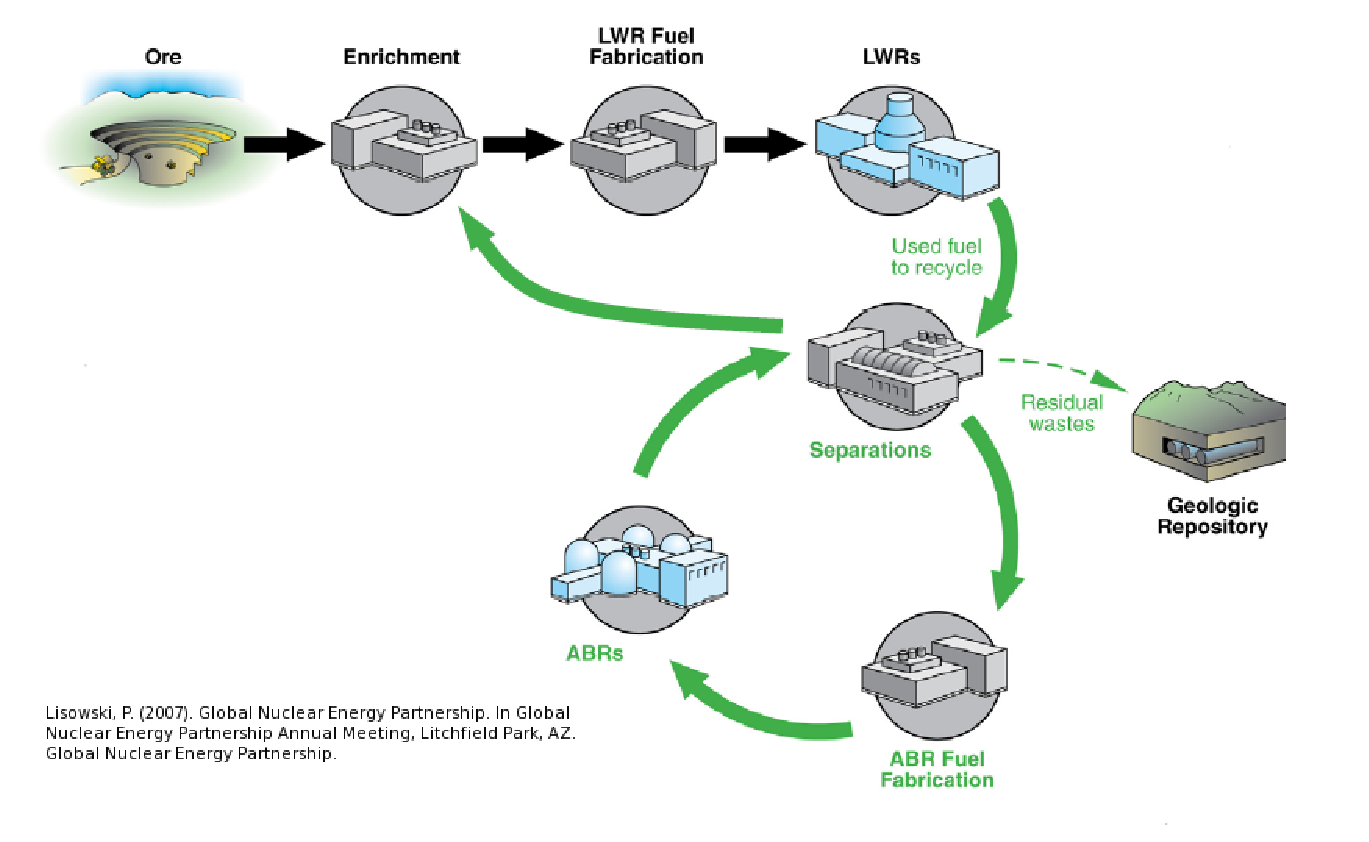
\includegraphics[height=4cm]{simulations.eps}
    \end{center}
    \caption{Top level simulators are intended to model the collective 
    behavior of various fuel cycle decisions and 
    strategies.\cite{lisowski_global_2007}}
    \label{fig:simulation}
  \end{figure}
\end{frame}
%---------------||||
\subsection{Lessons Learned}
%||||---------------
\begin{frame}[ctb!]
  \frametitle{Lessons Learned}
  Areas of unmet need in previous simulators include:
  \begin{itemize}
    \item \textbf{Usability} directed toward a wide range of user 
      sophistication.
    \item \textbf{Performance} solving simple problems in interactive time 
      scales
    \item \textbf{Fidelity} accommodating a range of levels of detail 
      commensurate with user sophistication
  \end{itemize}

  Valuable software development practices have been identified 
  \cite{huff_cyclus:_2010}\cite{huff_next_2010}: 
  \begin{itemize}
    \item{\textbf{Modularity}} allows the core infrastructure to be independent of 
      proprietary and/or sensitive data and/or models.
    \item{\textbf{Extensibility}} with a focus on both robustness and flexibility 
      allows for myriad potential developer extensions.
    \item{\textbf{Openness}} supports collaboration, verification, validation, 
      and code sustainability.
  \end{itemize}
\end{frame}
%---------------||||
%||||---------------
\begin{frame}
  \frametitle{Cyclus Modular Architecture and Open Development}
  The combination of modular encapsulation within the software
  architecture and an open development paradigm allows for collaboration
  at multiple levels of simulation detail and data security.
\end{frame}
%---------------||||

\section{Cyclus Modular Architecture}
\subsection{Model Hierarchy}
%||||---------------
\begin{frame}[ctb!]
  \frametitle{Region Institution Facility Hierarchy}
  \begin{figure}[hbtp!]
    \begin{center}
      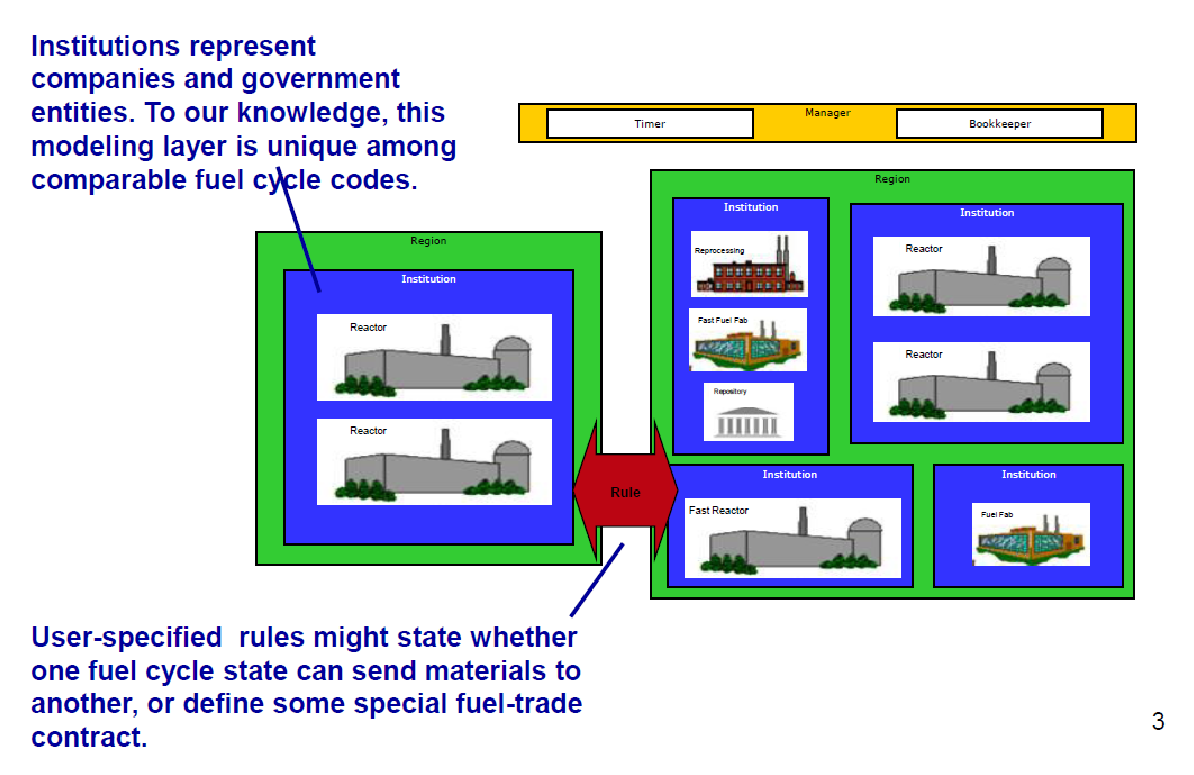
\includegraphics[height=4cm]{rif.eps}
    \end{center}
    \caption{The Region, Institution, Facility Hierarchy of the Cyclus 
    paradigm was a success of the GENIUSv2 
    code.\cite{oliver_geniusv2:_2009}}
    \label{fig:rif}
  \end{figure}
\end{frame}
%---------------||||
\subsection{Modularity}
%||||--------------
\begin{frame}[ctb!]
  \frametitle{Encapsulation}
  \begin{figure}[htbp!]
    \begin{center}
      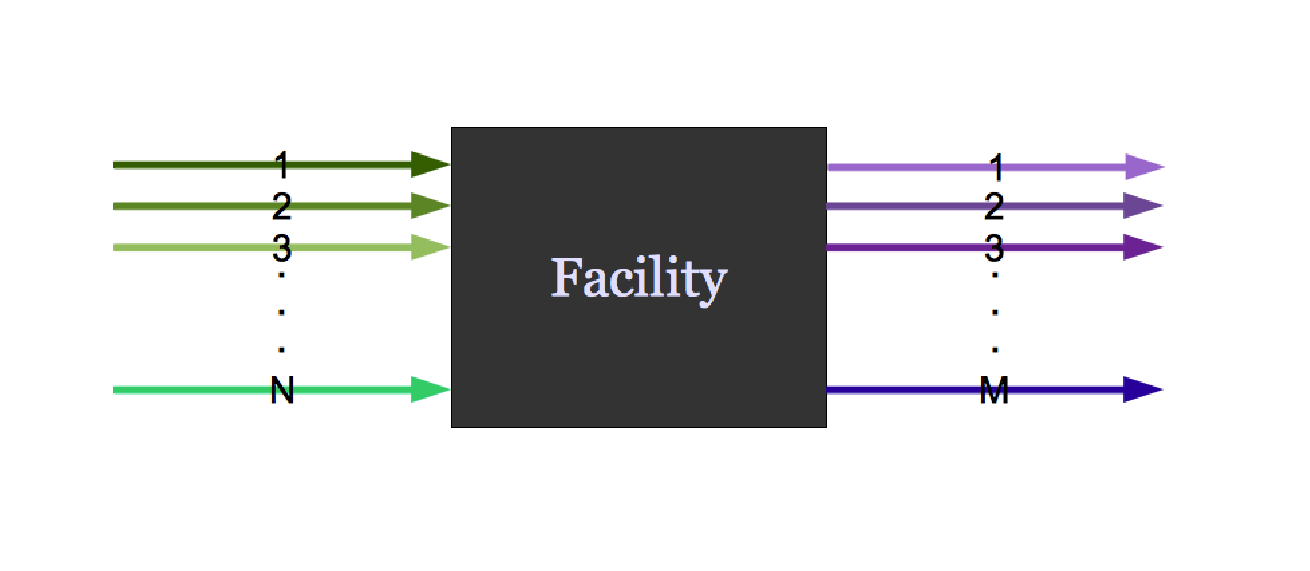
\includegraphics[height=5cm]{facility.eps}
    \end{center}
    \caption{ Regions, Institutions, Facilities, and Markets are all
    black boxes.} 
    \label{fig:sinkfacility}
  \end{figure}
\end{frame}
%---------------||||
%||||---------------
\begin{frame}[ctb!]
  \frametitle{Module Interfaces}
  \begin{figure}[htbp!]
    \begin{center}
      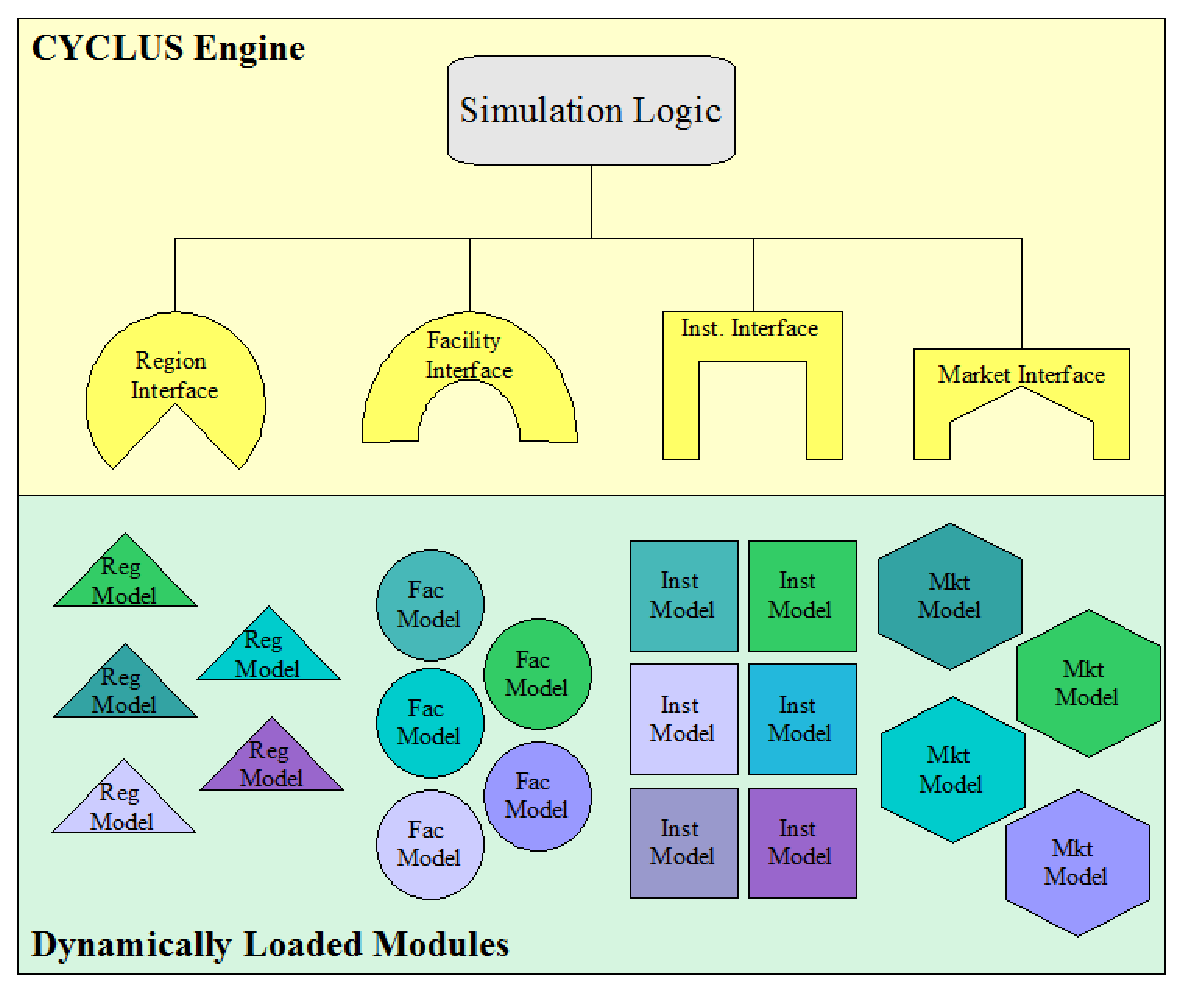
\includegraphics[height=5cm]{interfaces.eps}
    \caption{Well defined model interfaces facilitate model 
    interchange. The user may choose the model at their desired level  
    of detail.}
    \label{fig:interfaces}
    \end{center}
  \end{figure}
\end{frame}
%---------------||||

%||||---------------
\begin{frame}[ctb!]
  \frametitle{Facilities Are Black Boxes}
  \begin{figure}[htbp!]
    \begin{center}
      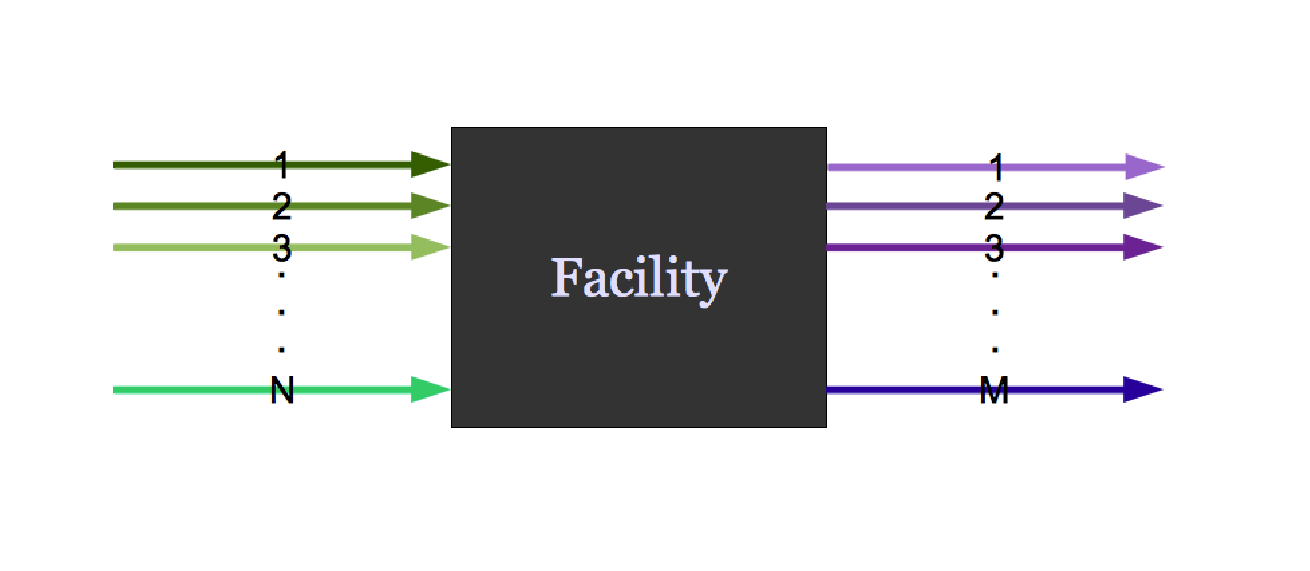
\includegraphics[height=5cm]{facility.eps}
    \end{center}
    \caption{ Each facility in the simulation makes requests and offers 
    to fill its stocks and empty its inventory respectively.  }
    \label{fig:facility}
  \end{figure}
\end{frame}
%---------------||||
\subsection{Example : Market-Facility Interface}
%||||--------------
\begin{frame}[ctb!]
  \frametitle{Facilities Are Black Boxes}
  \begin{figure}[htbp!]
    \begin{center}
      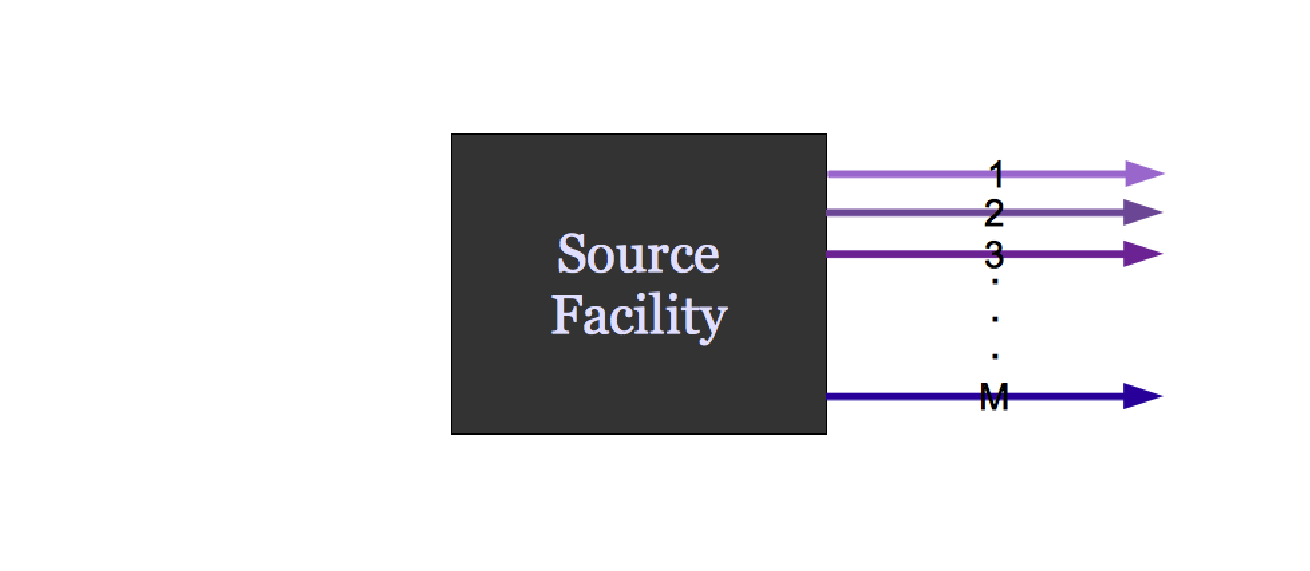
\includegraphics[height=5cm]{sourcefacility.eps}
    \end{center}
    \caption{ A facility might only make offers.} 
    \label{fig:sourcefacility}
  \end{figure}
\end{frame}
%---------------||||
%||||--------------
\begin{frame}[ctb!]
  \frametitle{Facilities Are Black Boxes}
  \begin{figure}[htbp!]
    \begin{center}
      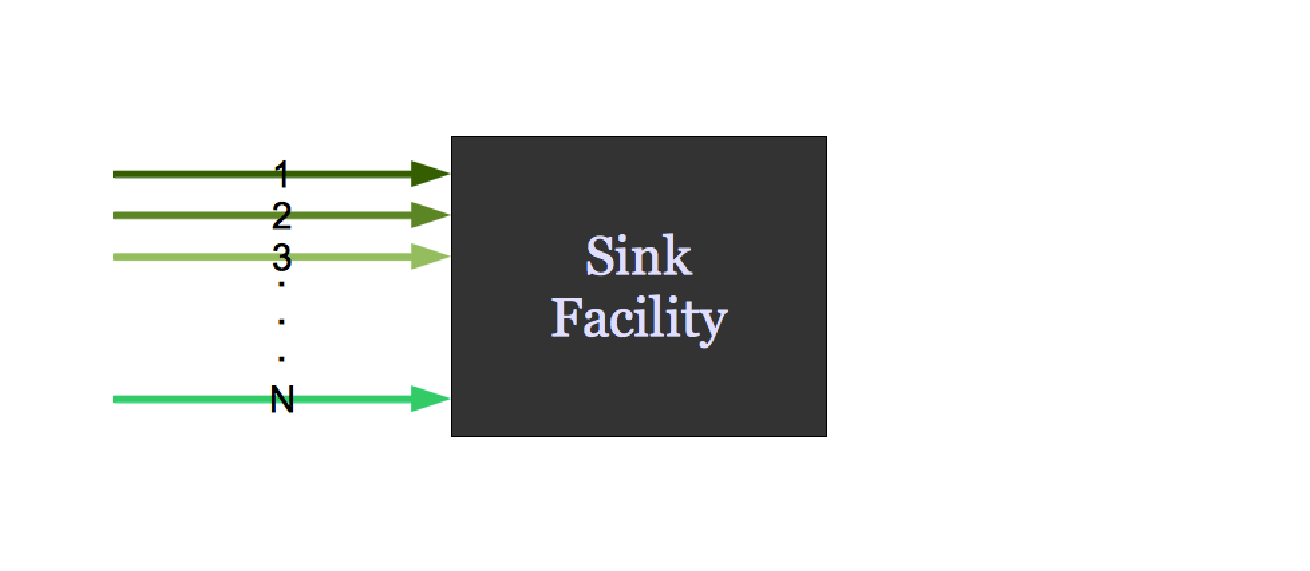
\includegraphics[height=5cm]{sinkfacility.eps}
    \end{center}
    \caption{ A facility might only make requests.} 
    \label{fig:sinkfacility}
  \end{figure}
\end{frame}
%---------------||||
%||||--------------
\begin{frame}[ctb!]
  \frametitle{Each Commodity is Associated with a Market}
  \begin{figure}[htbp!]
    \begin{center}
      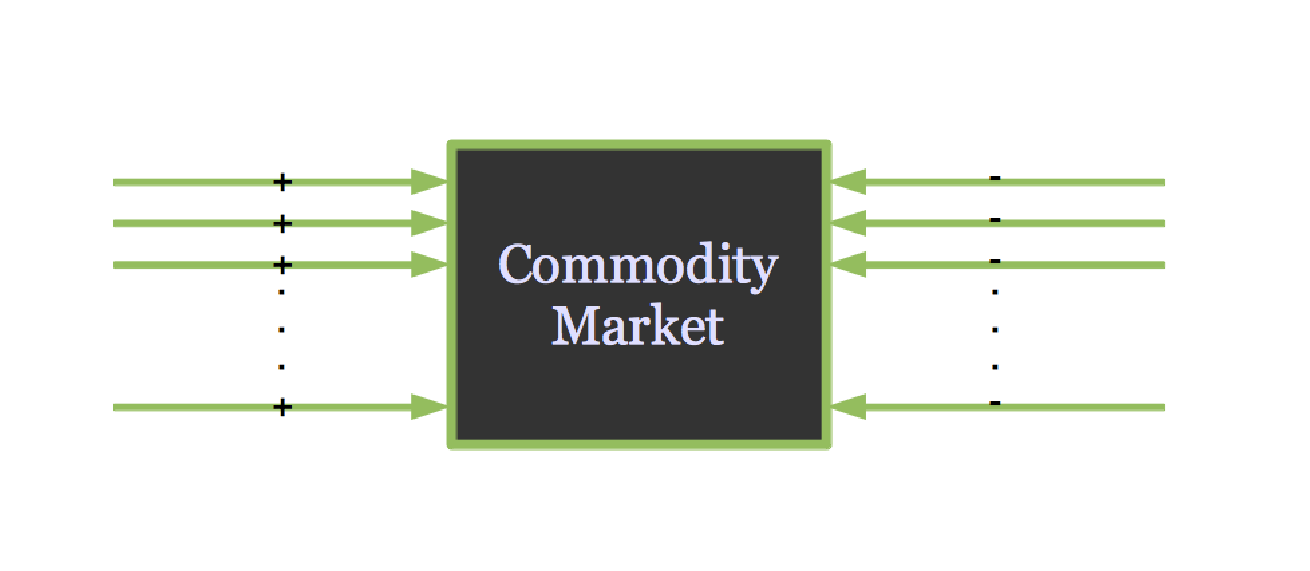
\includegraphics[height=5cm]{market.eps}
    \end{center}
    \caption{ A market receives offers and requests concerning its 
    commodity. } 
    \label{fig:market}
  \end{figure}
\end{frame}
%---------------||||
%||||--------------
\begin{frame}[ctb!]
  \frametitle{The Market Solves the Matching Problem}
  \begin{figure}[htbp!]
    \begin{center}
      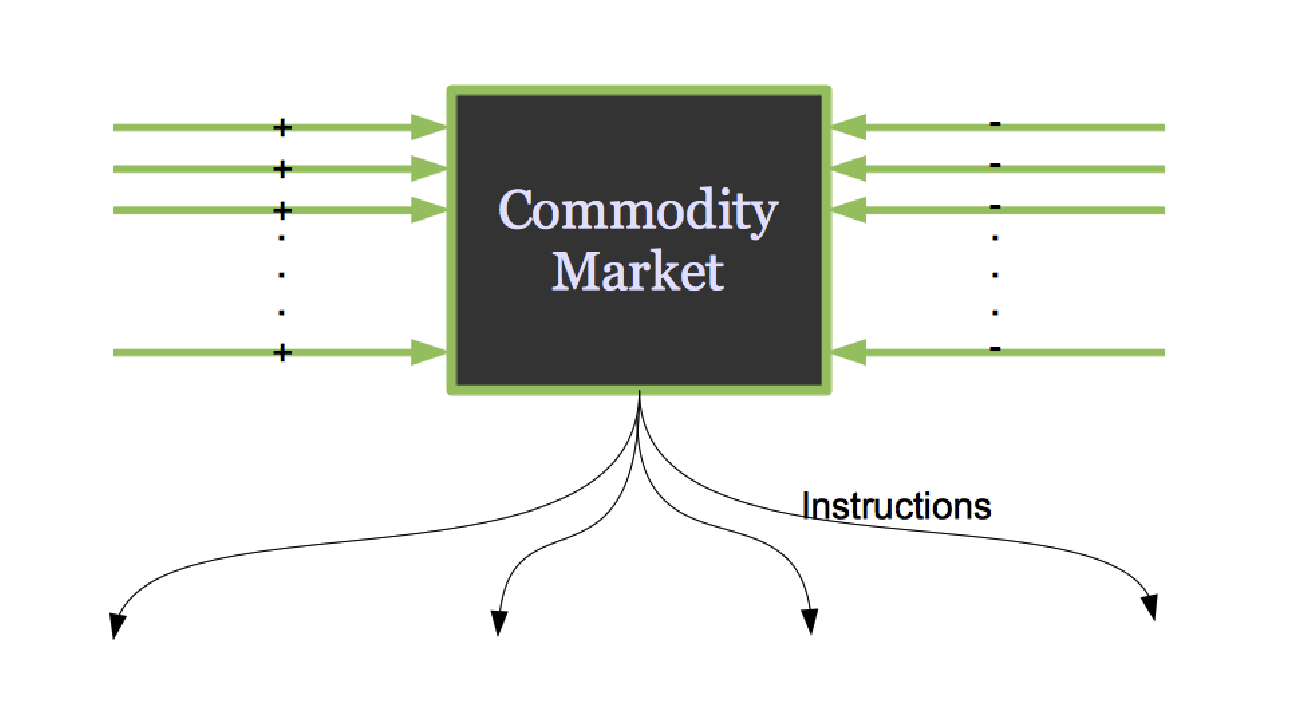
\includegraphics[height=5cm,width=8cm]{instructions.eps}
    \end{center}
    \caption{ When the Market's arbitrary algorithm solves the 
    matching problem, the Market sends instructions to the offering 
    facilities.} 
    \label{fig:instructions}
  \end{figure}
\end{frame}
%---------------||||
%||||--------------
\begin{frame}[ctb!]
  \frametitle{A Simple Example}
  \begin{figure}[htbp!]
    \begin{center}
      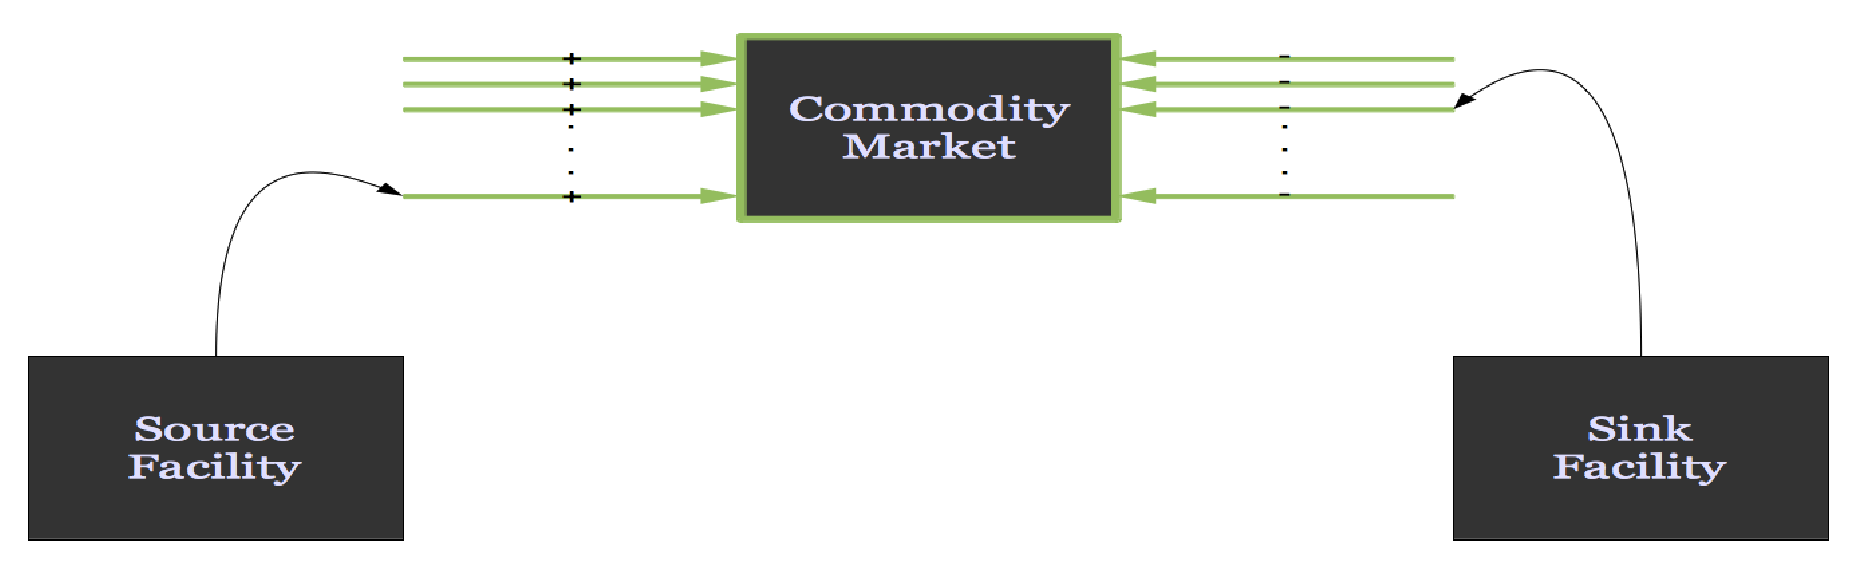
\includegraphics[height=5cm, width=8cm]{offreq.eps}
    \end{center}
    \caption{ The source sends an offer and the sink sends a request.} 
    \label{fig:offreq}
  \end{figure}
\end{frame}
%---------------||||
%||||--------------
\begin{frame}[ctb!]
  \frametitle{A Simple Example}
  \begin{figure}[htbp!]
    \begin{center}
      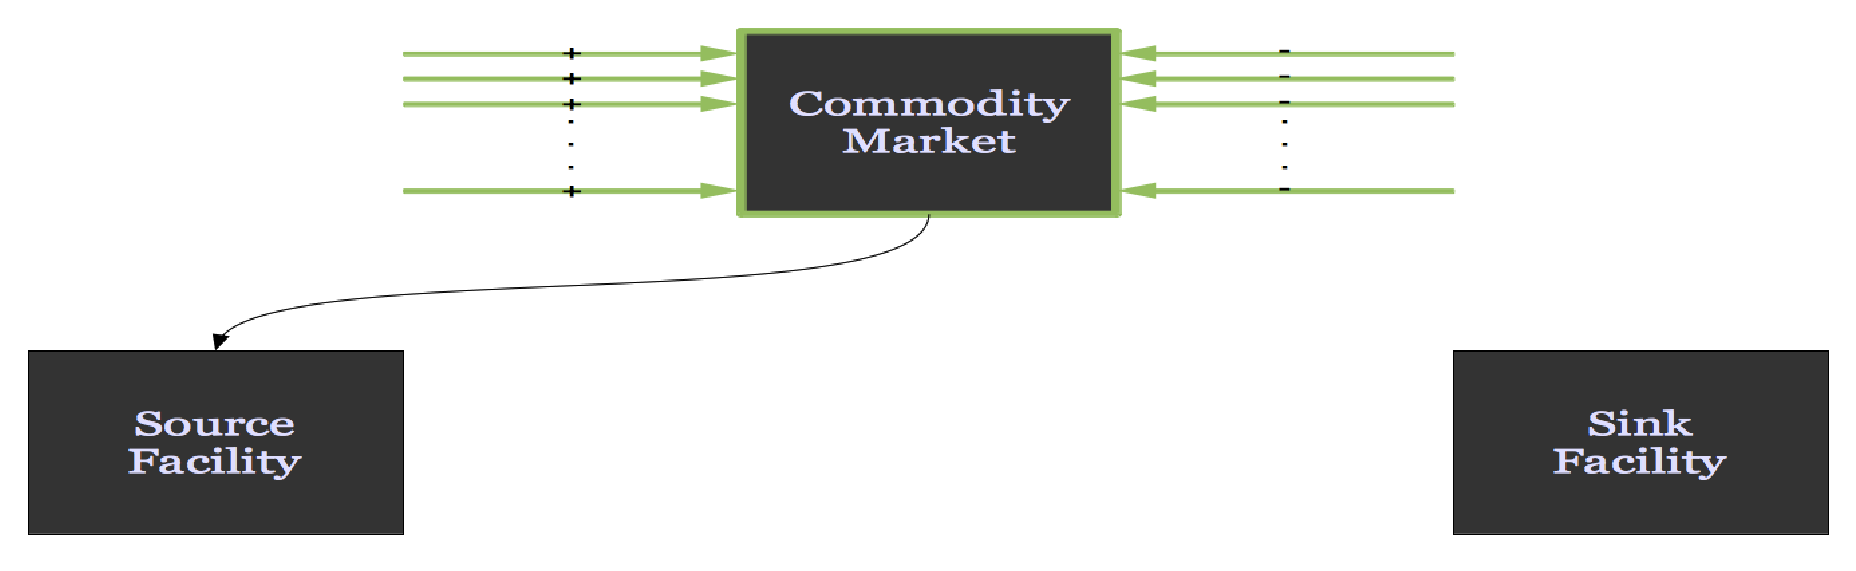
\includegraphics[height=5cm, width=8cm]{transmess.eps}
    \end{center}
    \caption{ The Market solves the problem and instructs the source 
    facility to send a certain amount to the sink facility.} 
    \label{fig:transmess}
  \end{figure}
\end{frame}
%---------------||||
%||||--------------
\begin{frame}[ctb!]
  \frametitle{A Simple Example}
  \begin{figure}[htbp!]
    \begin{center}
      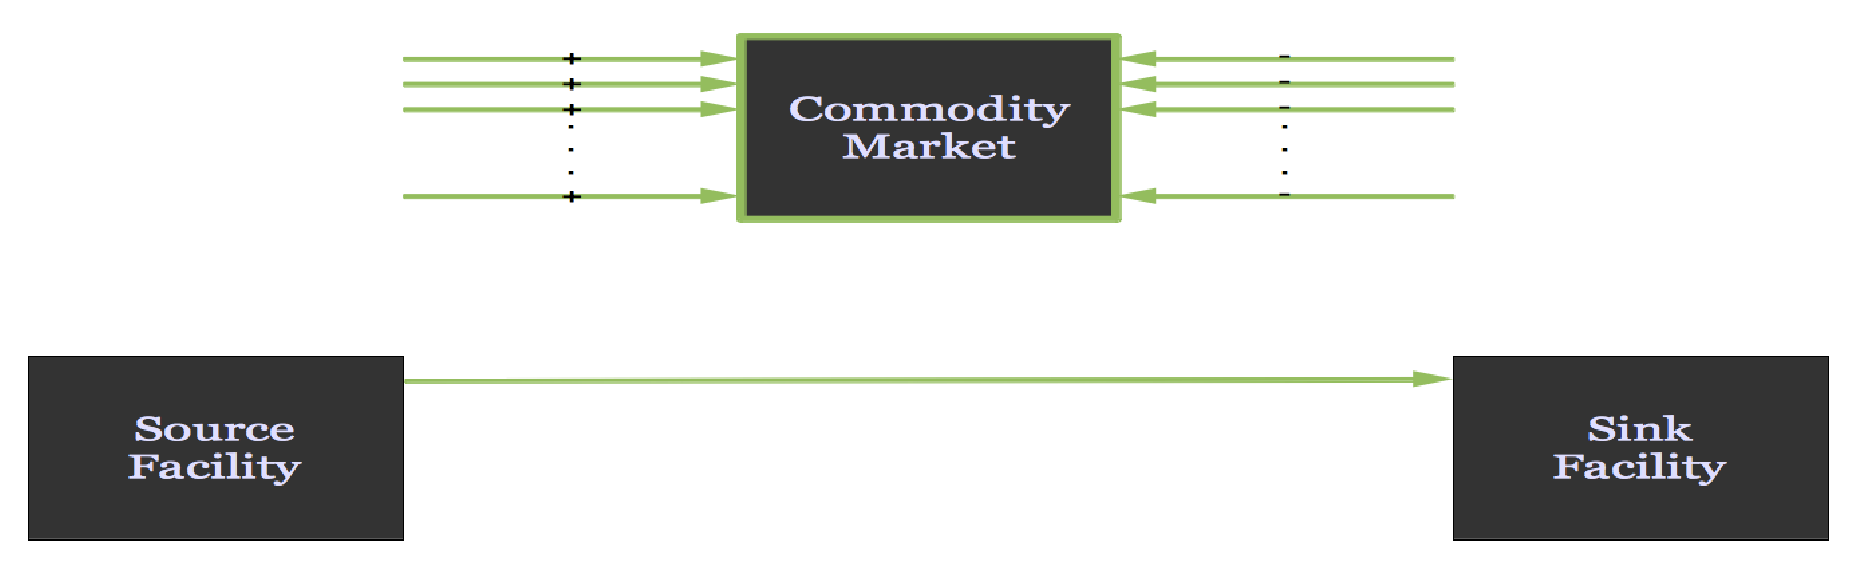
\includegraphics[height=5cm, width=8cm]{trans.eps}
    \end{center}
    \caption{ The source facility sends the material directly to the 
    sink facility.} 
    \label{fig:trans}
  \end{figure}
\end{frame}
%---------------||||
%||||---------------
\begin{frame}[ctb!]
  \frametitle{This Market Model Scales for Complex Systems}
  \begin{figure}[htbp!]
    \begin{center}
      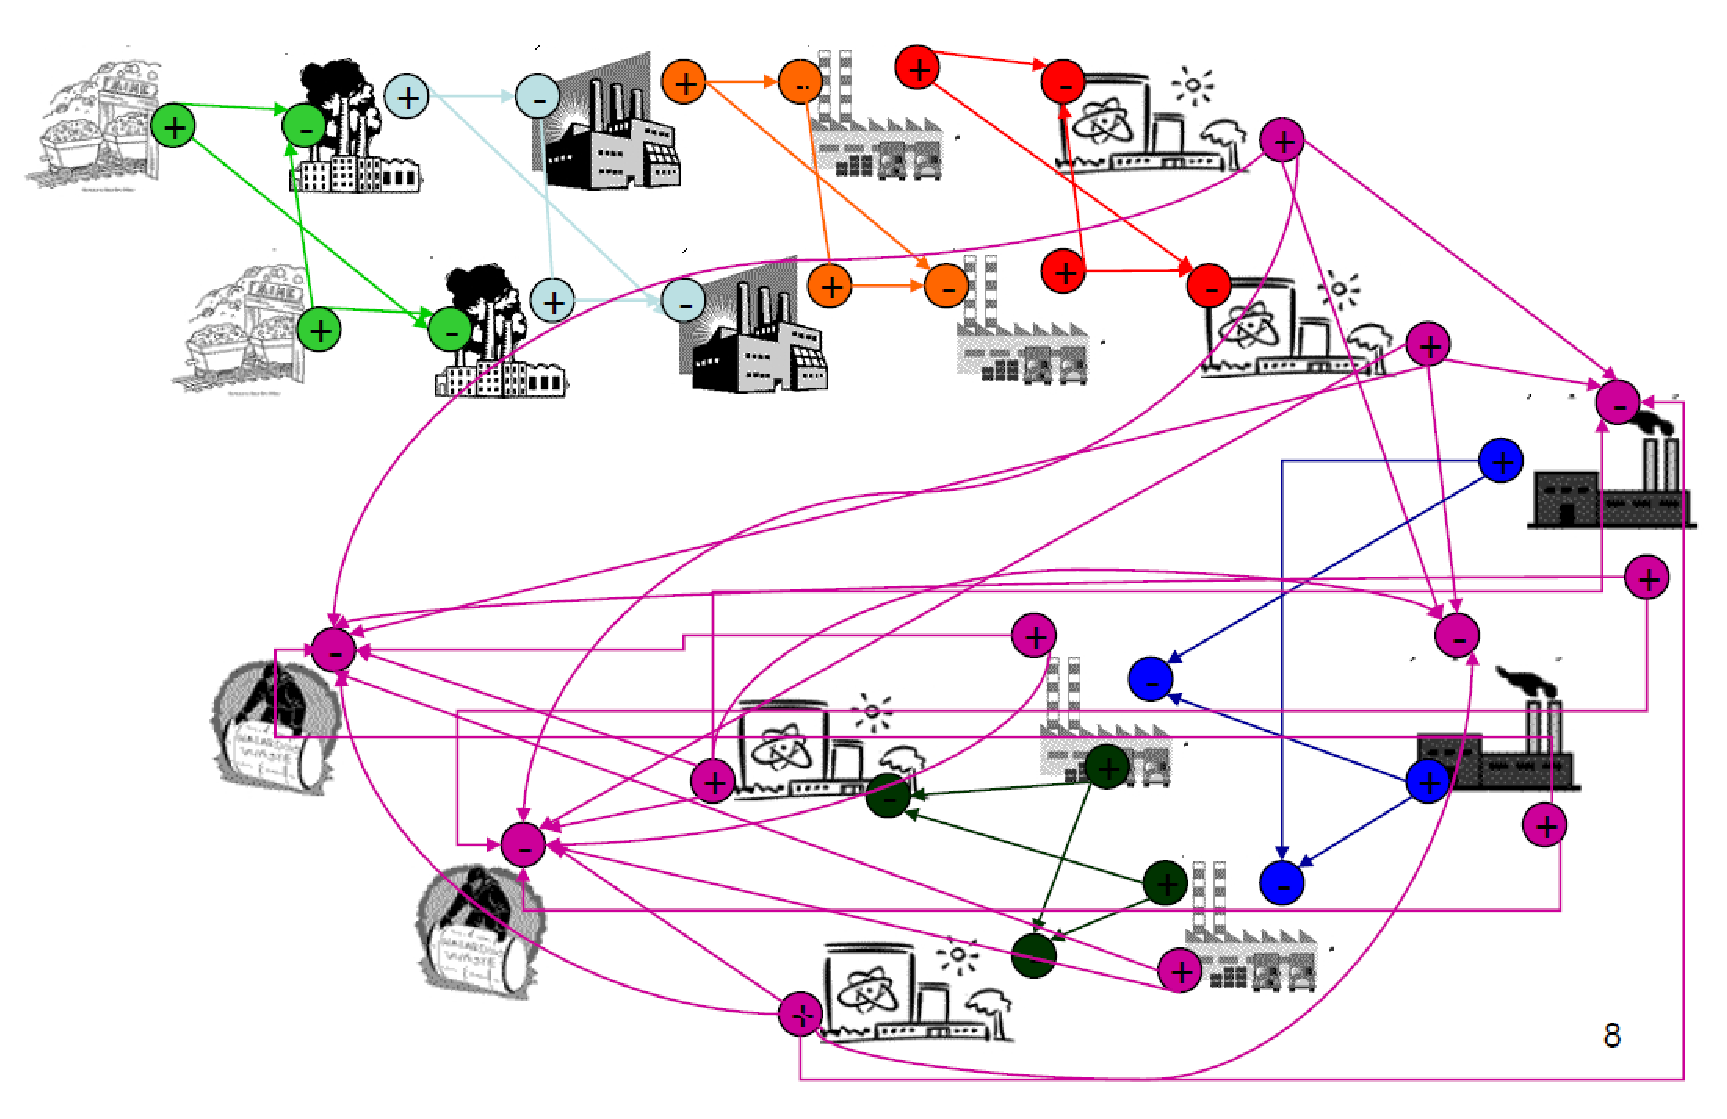
\includegraphics[height=6cm]{materials.eps}
    \end{center}
    \caption{Well designed interfaces and strict encapsulation support 
    scalability of the Market-based simulation paradigm 
    \cite{oliver_geniusv2:_2009}}
    \label{fig:materials}
  \end{figure}
\end{frame}
%---------------||||


\subsection{Extensibility}
%||||---------------
\begin{frame}
  \frametitle{Dynamic Module Loading : Developer}
  With a dynamic, plug-in implementation, the simulation logic is 
  independent of the available models and models are loaded as shared 
  libraries at runtime. 

  \begin{figure}[htbp!]
    \begin{center}
      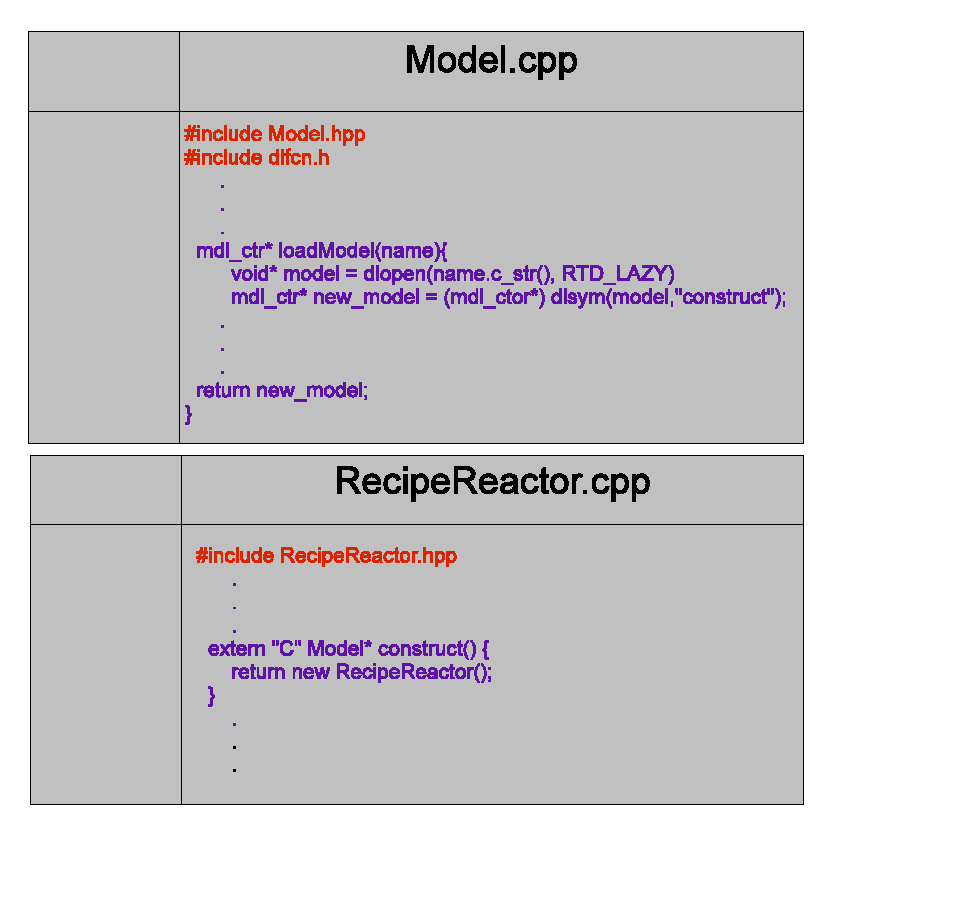
\includegraphics[height=5.5cm]{developer.eps}
    \end{center}
    \caption{Dynamic c library loading separates simulation logic from 
    knowledge of available models, supporting extensions by developers 
    with minimal lines of code.}
    \label{fig:xmlinput}
  \end{figure}

\end{frame}
%---------------||||
%|||---------------
\begin{frame}[ctb!]
  \frametitle{Cross Platform, Multi-language}
  CMake (Crossplatform Make) build system is cross platform. Thus, 
  users may build and run Cyclus on Windows, Mac, or Linux 
  operating systems. 
  
  CMake is also multilingual, so modules may be written in any language 
  or tool that can be made into a shared object library or wrapped 
  with C++. 

  These include (but are not limited to): 
  \begin{itemize}
    \item Fortran
    \item Python
    \item R
    \item Java
    \item Lisp
    \item IDL
    \item Matlab
    \item Perl
    \item etc\ldots
  \end{itemize}
\end{frame}
%---------------||||
%||||---------------
\begin{frame}[ctb!]
  \frametitle{Dynamic Module Loading : User}
  With a dynamic, plug-in implementation, the simulation logic is 
  independent of the available models and models are loaded as shared 
  libraries at runtime. 

  \begin{figure}[htbp!]
    \begin{center}
      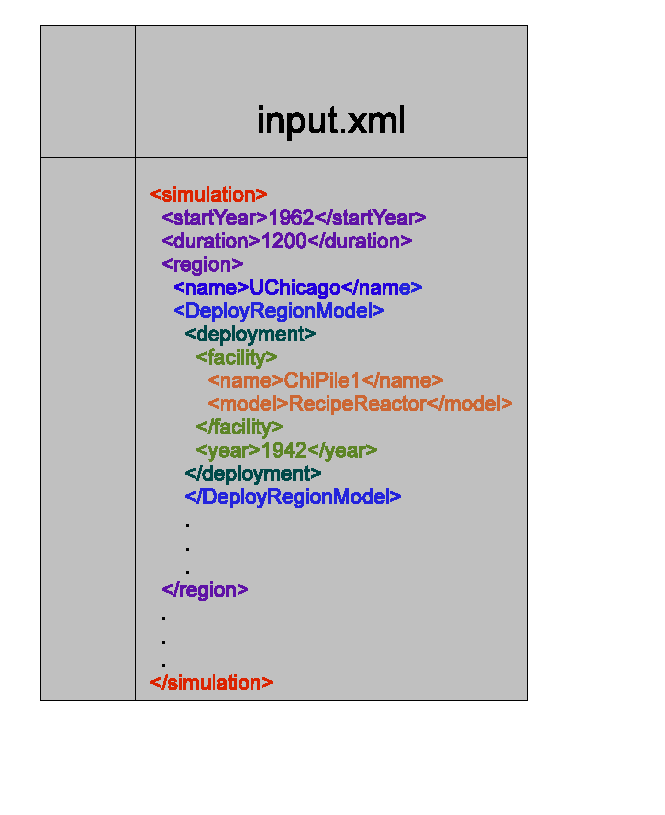
\includegraphics[height=5.5cm]{user.eps}
    \end{center}
    \caption { XML input parsing and a relaxNG schema provide 
    a simplified XML interface is available for the end
    user to define available module implementations.  }
    \label{fig:xmlinput}
  \end{figure}

\end{frame}
%---------------||||

\section{Cyclus Development Paradigm}
\subsection{ ` Modified Open' Source}
%||||---------------
\begin{frame}[ctb!]
  \frametitle{Open Source Repository}
    This open source repository provides a centralized location for 
    documentation, developer history, and unhindered developer access.
  \begin{figure}[htbp!]
    \begin{center}
      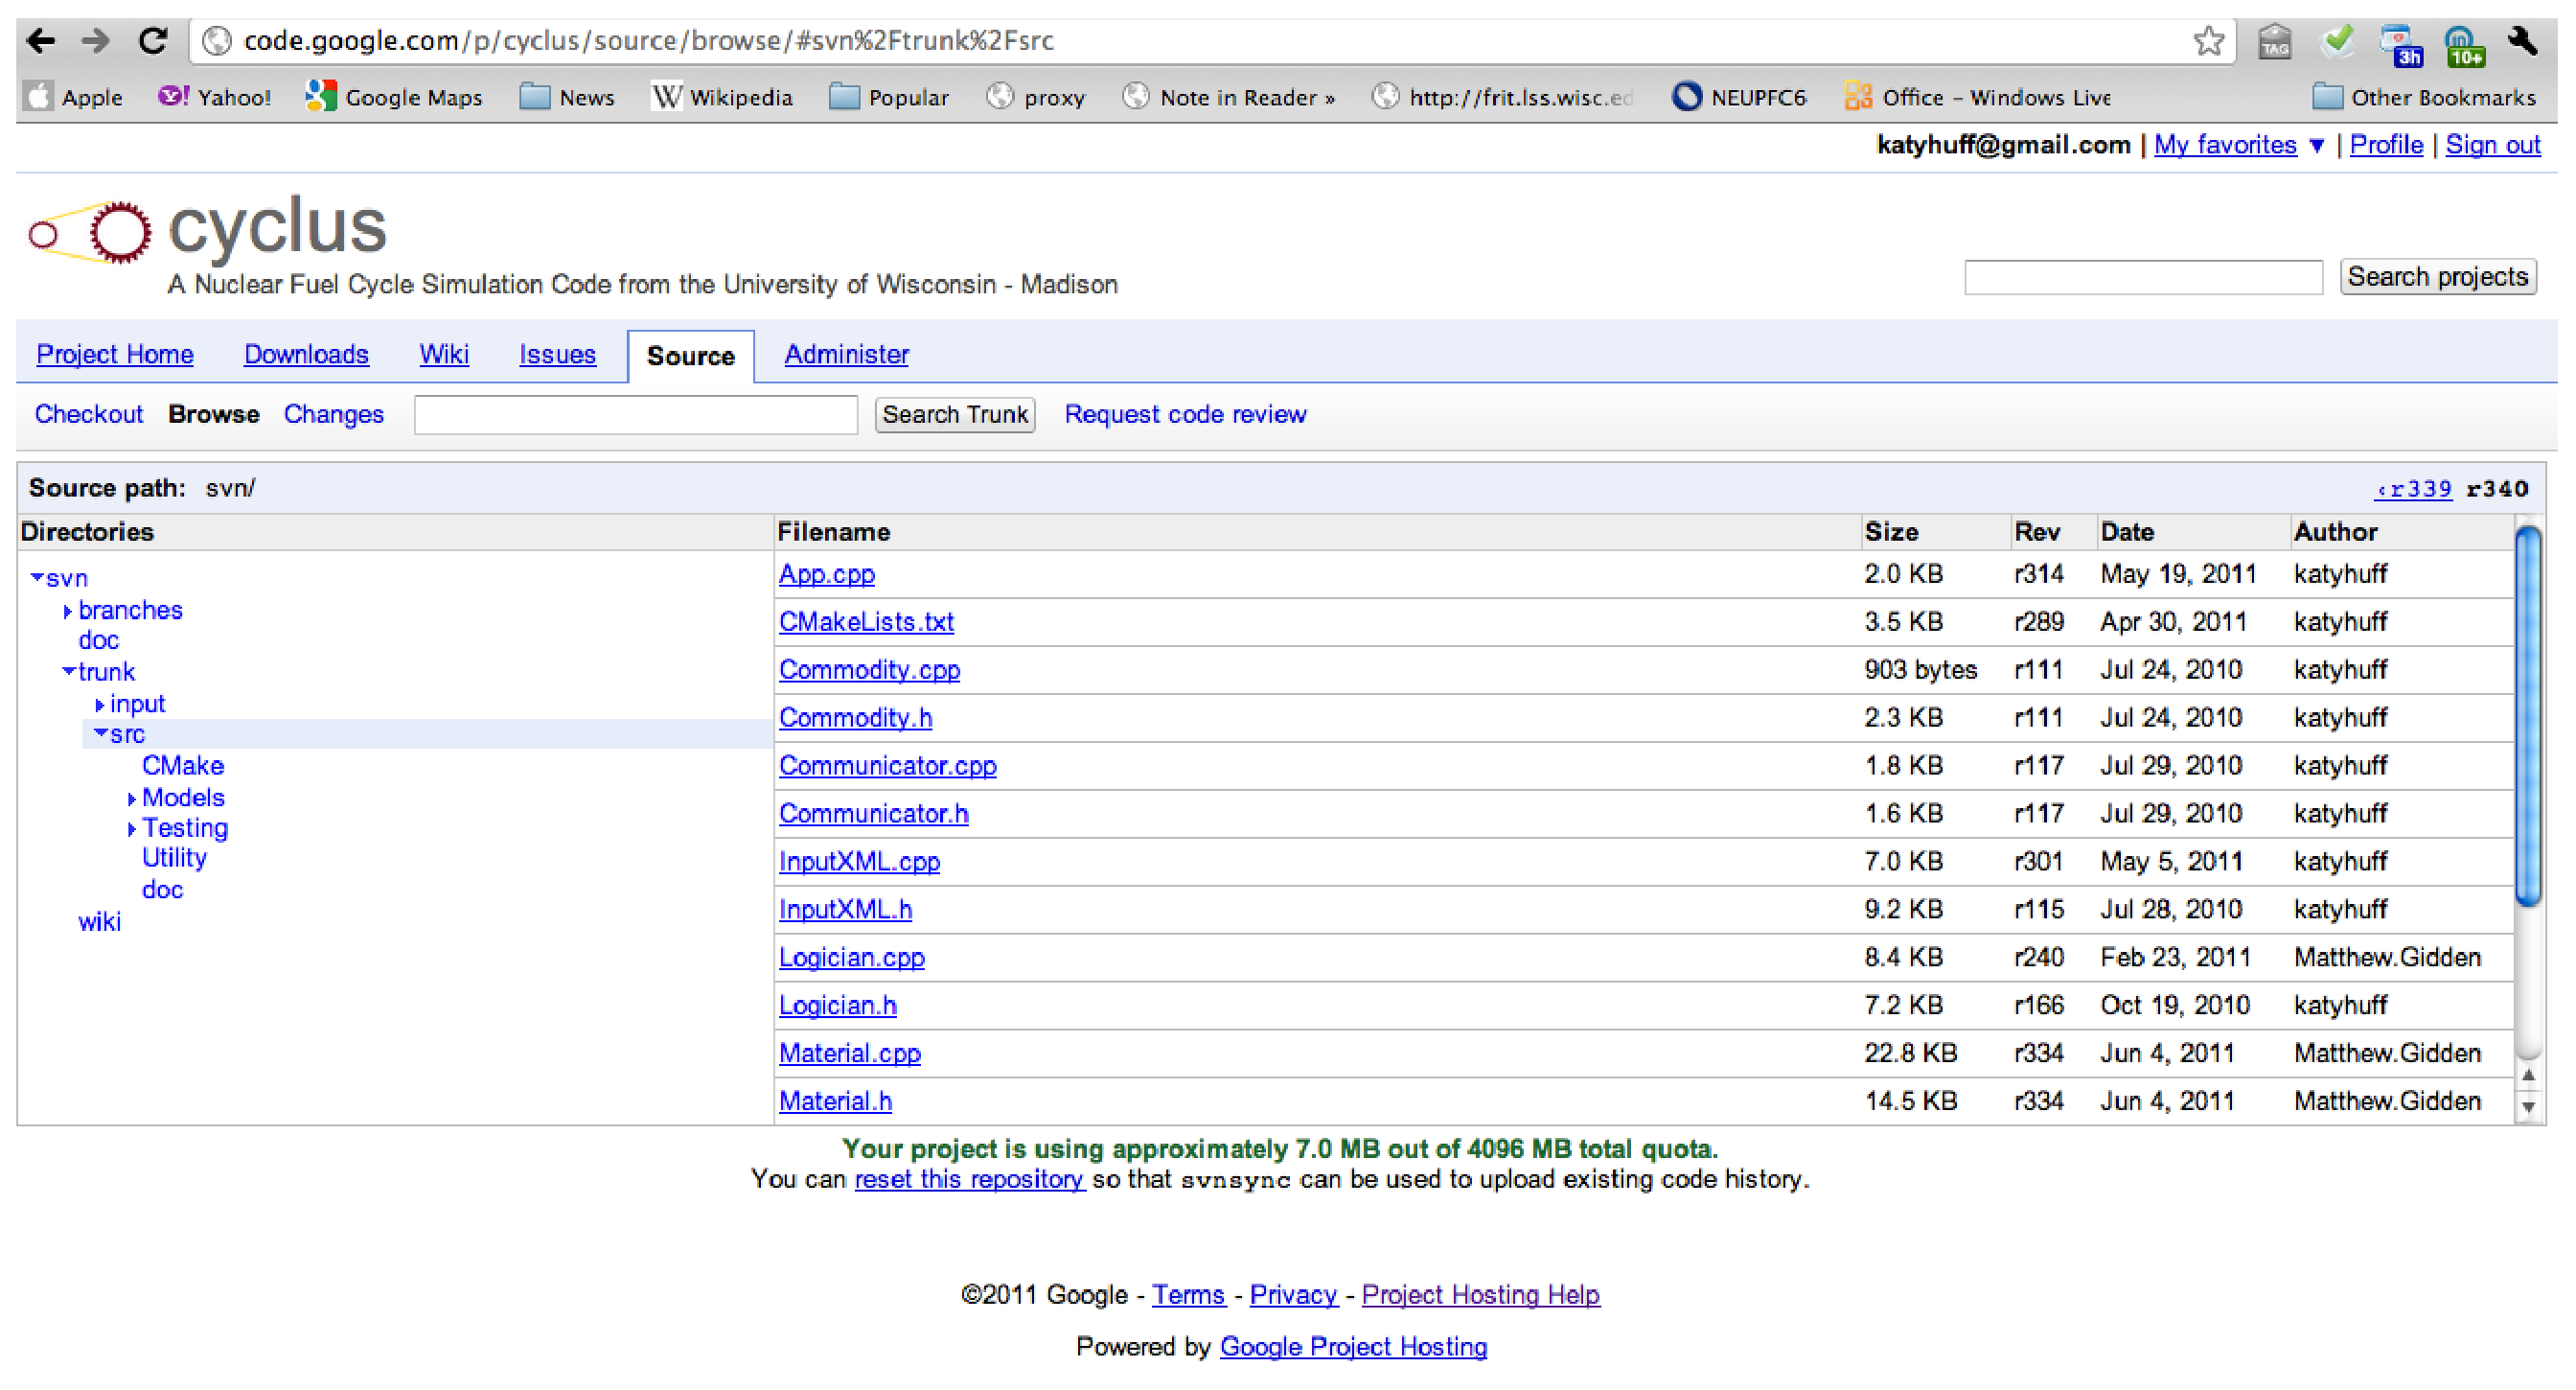
\includegraphics[height=6cm]{source.eps}
    \end{center}
    \caption{The current source code, complete revision history, and 
    documentation are made available for download and contribution 
    online. }
    \label{fig:open}
  \end{figure}
\end{frame}
%---------------||||
%||||---------------
\begin{frame}[ctb!]
  \frametitle{ `Modified Open' Source}
  \begin{figure}[hbtp!]
    \begin{center}
      
\includegraphics[height=6cm]{security.eps}
    \end{center}
    \caption{License, architecture, and development paradigm allow 
    varying levels of code sharing and data security.}
    \label{fig:security}
  \end{figure}
\end{frame}
%---------------||||
\subsection{Quality Control}
%||||---------------
\begin{frame}[ctb!]
  \frametitle{Version Control}
    This open source repository employs a version control system 
     for provenance, developer access, and reproducibility of results.
  \begin{figure}[htbp!]
    \begin{center}
      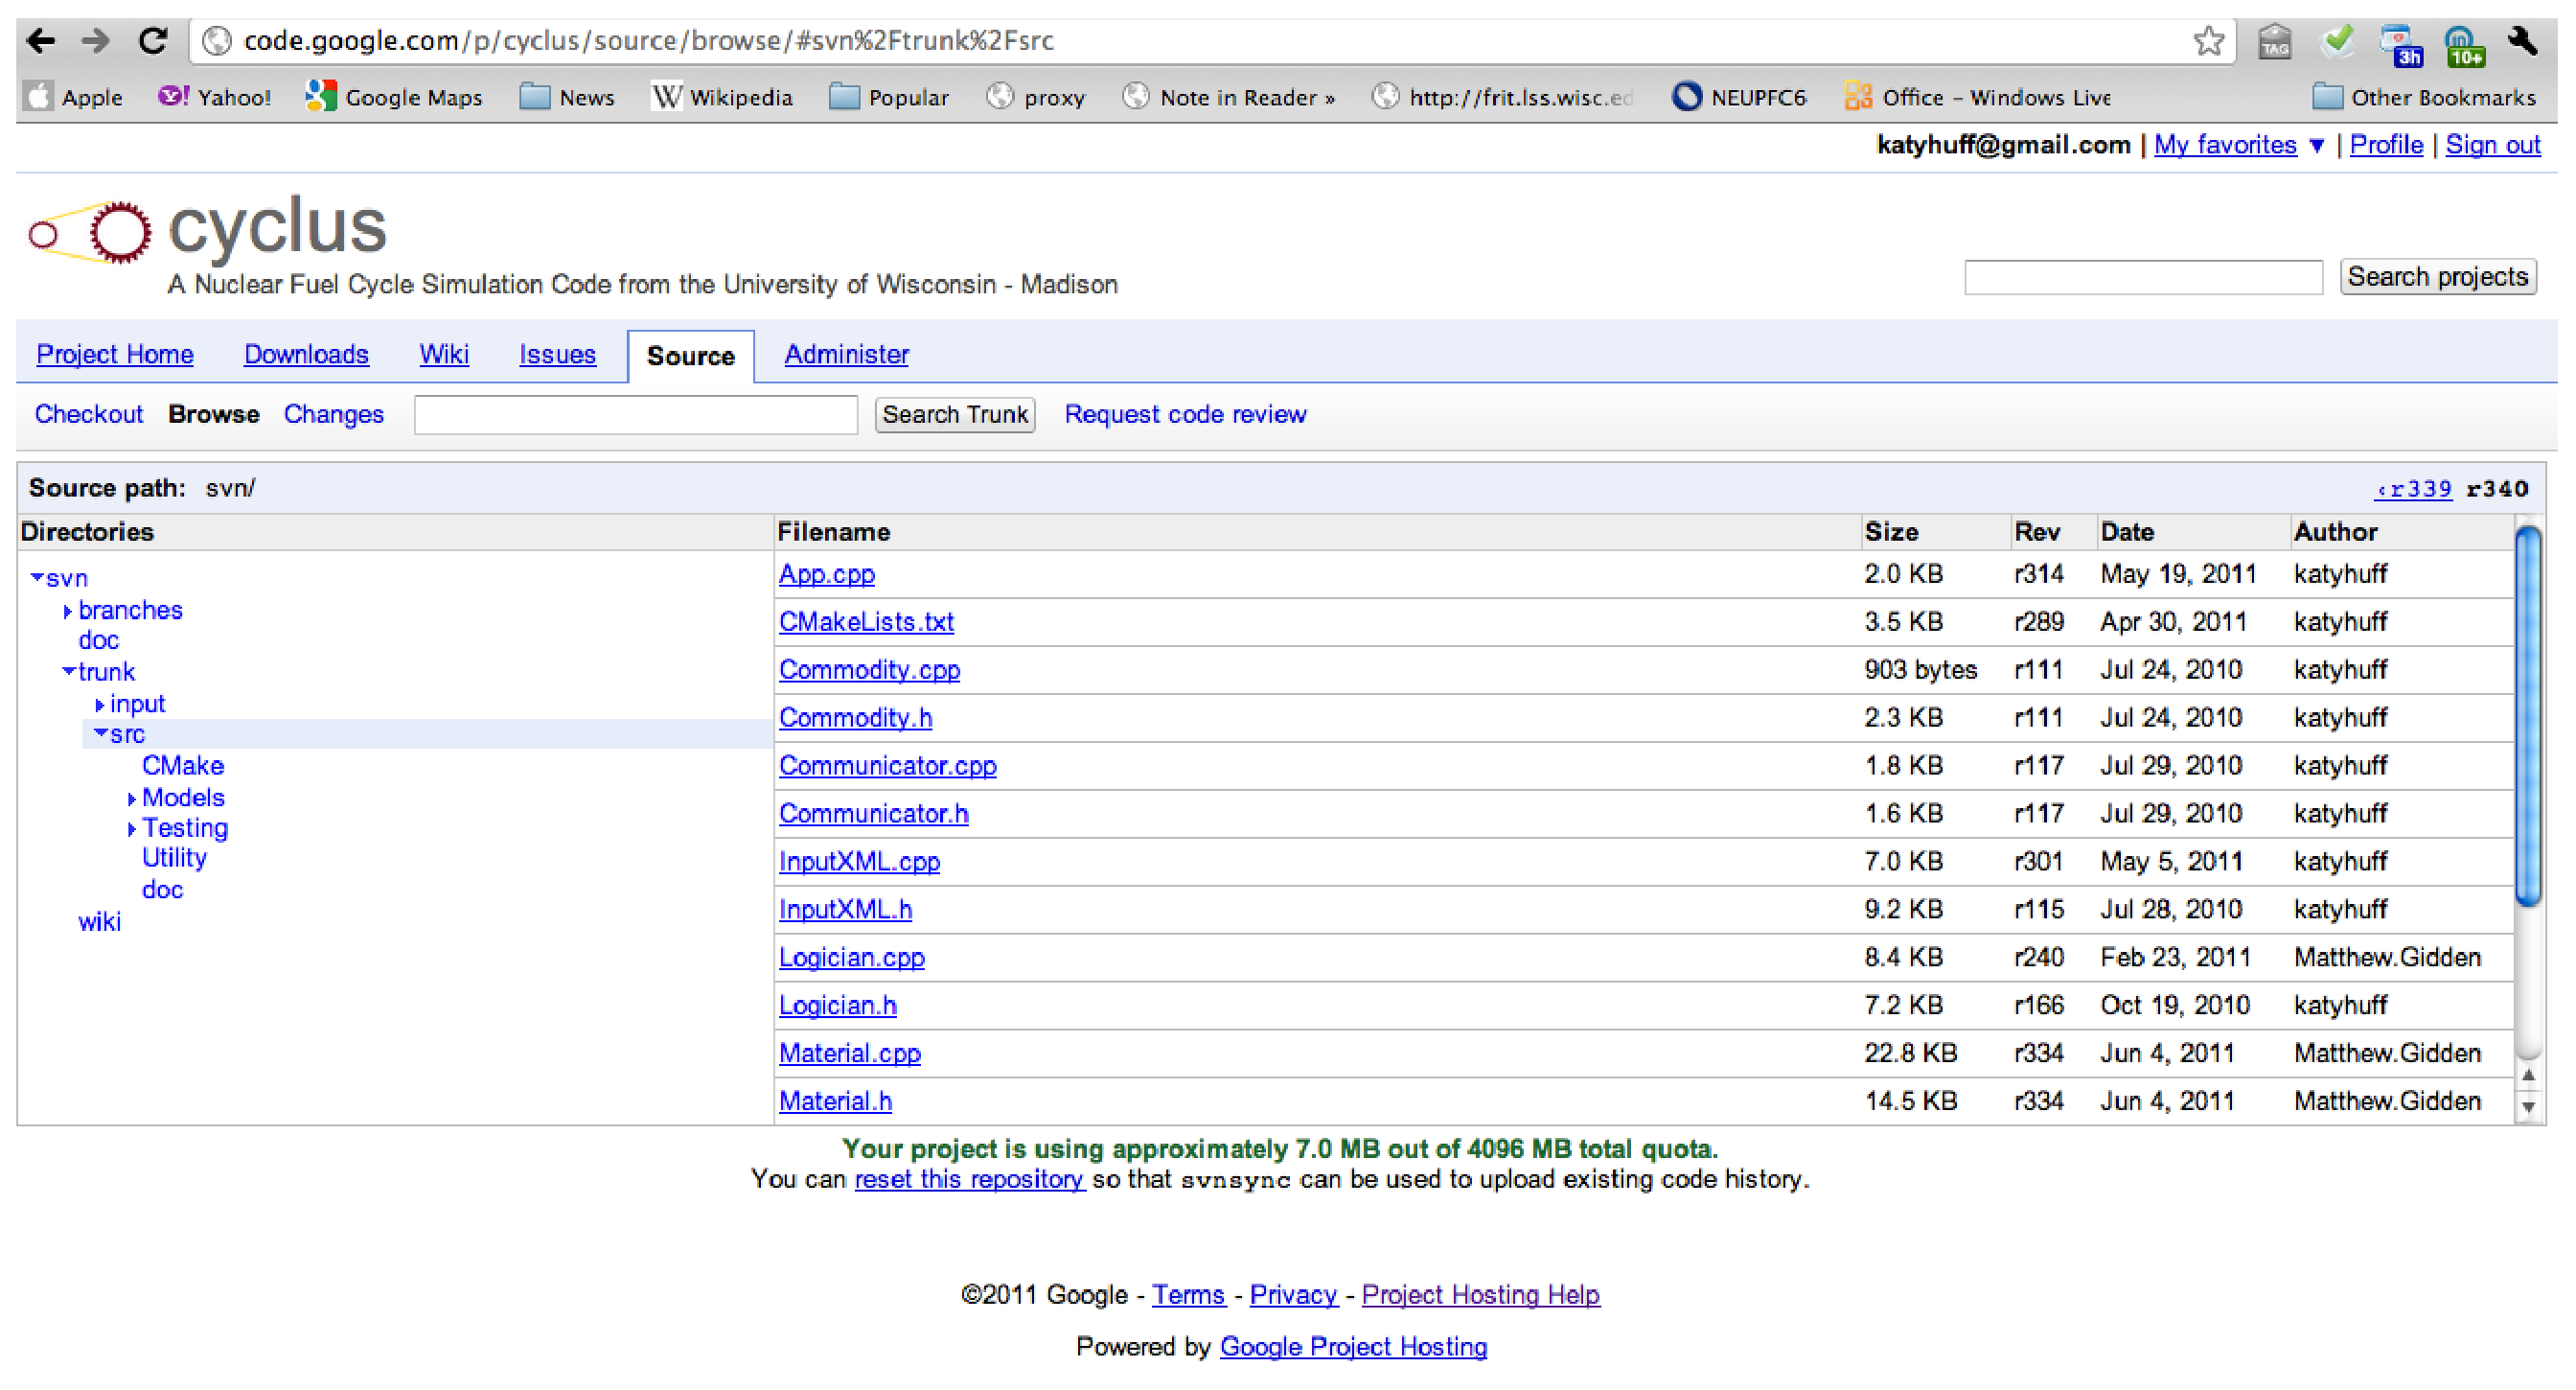
\includegraphics[height=6cm]{source.eps}
    \end{center}
    \caption{The current source code, commit messages, and complete 
    revision history is recorded and available in the repository.}
    \label{fig:source}
  \end{figure}
\end{frame}
%---------------||||
%||||---------------
\begin{frame}[ctb!]
  \frametitle{Issue Tracking}
    A built-in issue tracking system allows ticketing of 
    development milestones and public bug reporting.
  \begin{figure}[htbp!]
    \begin{center}
      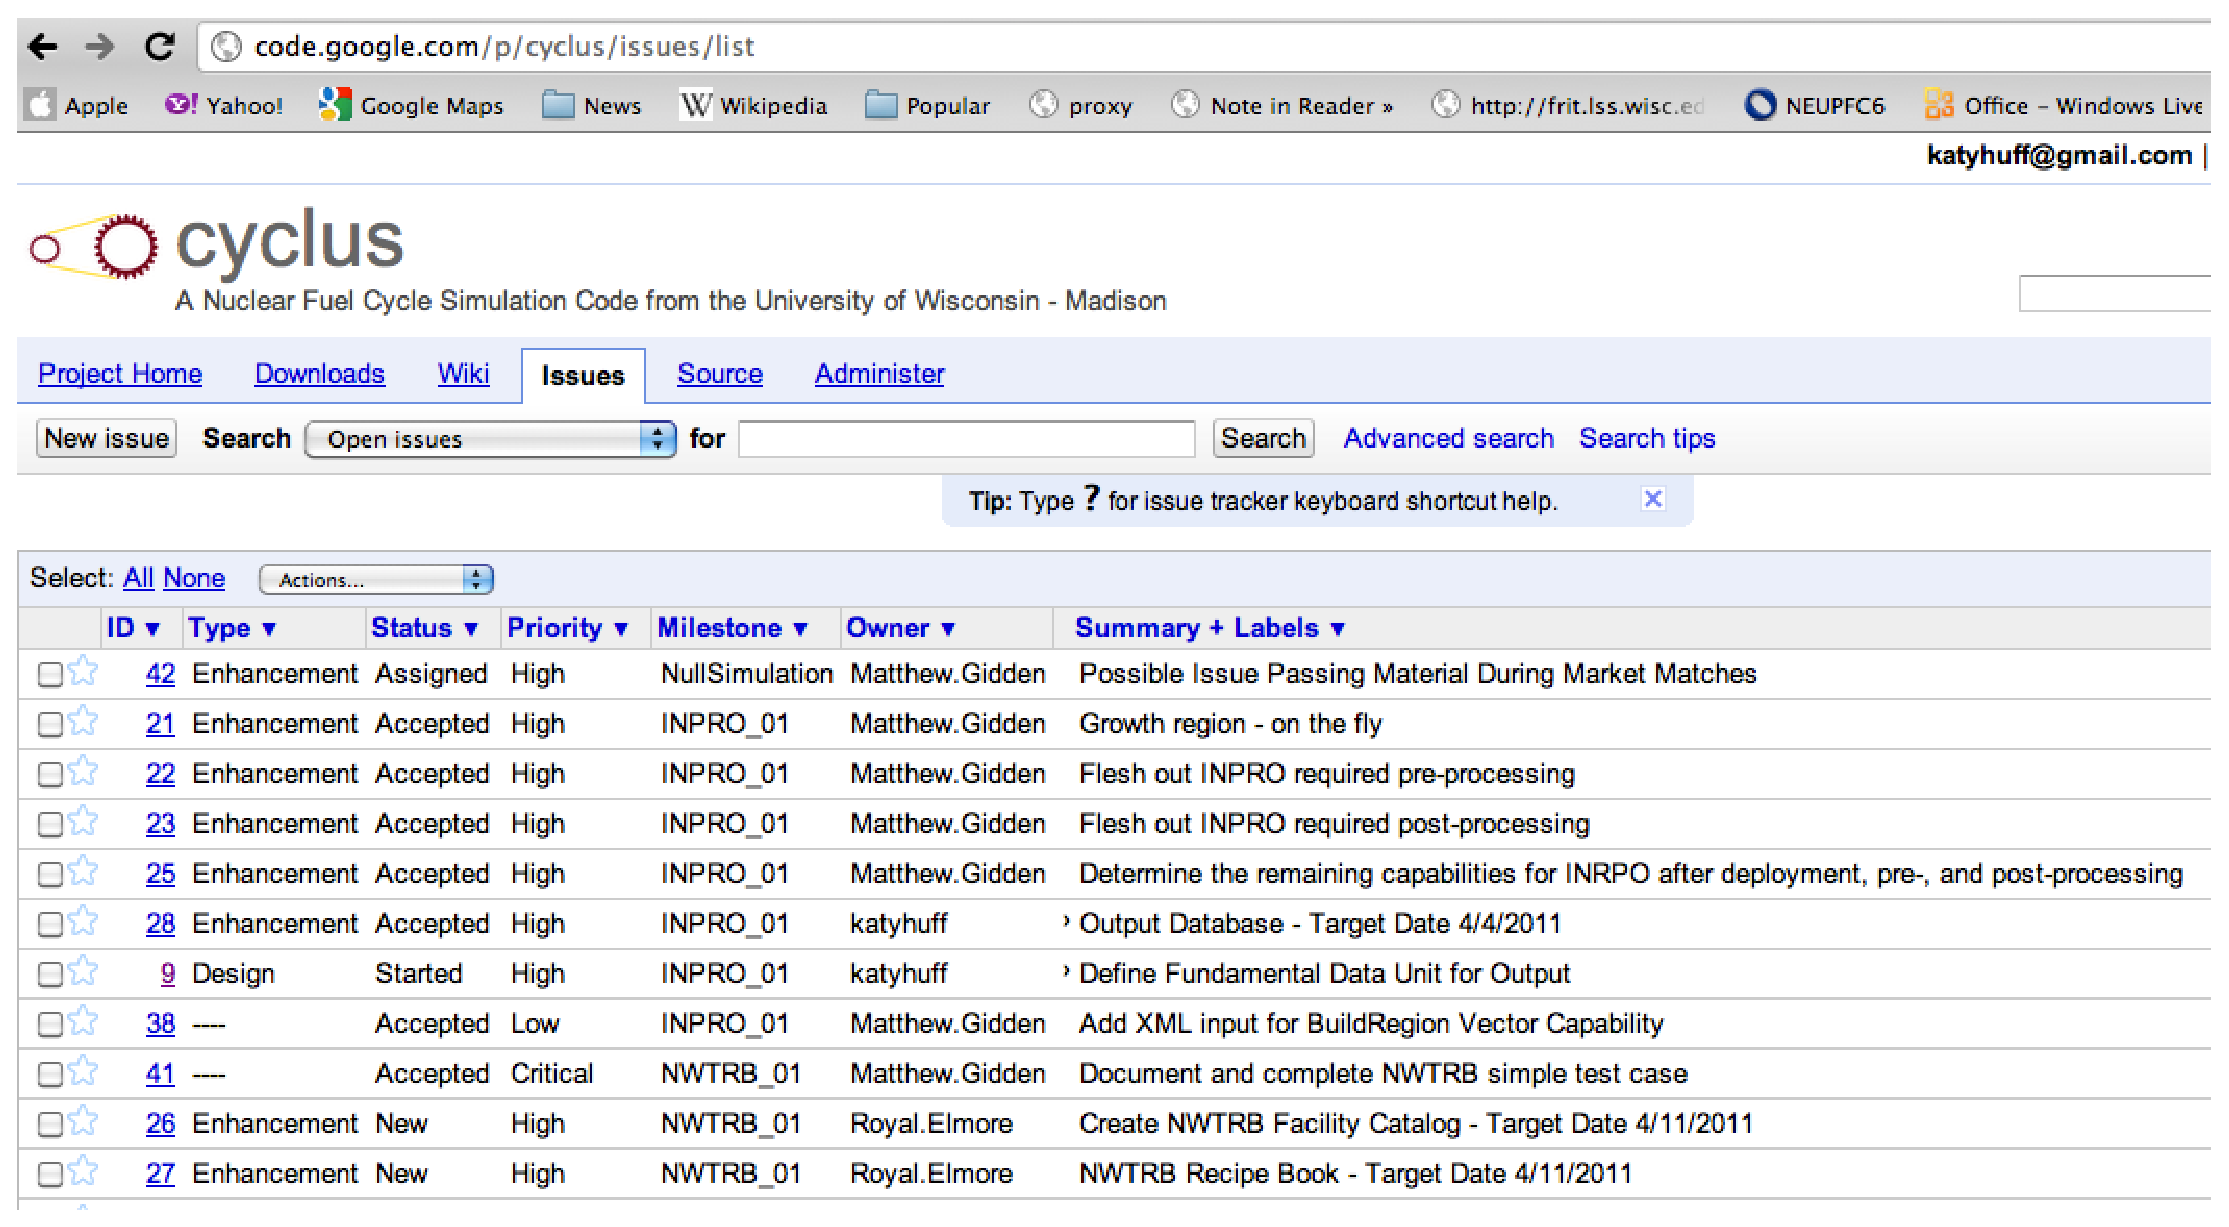
\includegraphics[height=6cm]{issues.eps}
    \end{center}
    \caption{ Issues are created, assigned, and kept track of 
    alongside the code. } 
    \label{fig:issues}
  \end{figure}
\end{frame}
%---------------||||
%||||---------------
\begin{frame}[ctb!]
  \frametitle{Collaborative Verification}
  The \textbf{transparency} inherent in this type of open source 
    development path also \textbf{facilitates code review}
    by exposing available content to verification and validation 
    \textbf{by collaborators} with diverse areas of specialization and levels 
    of expertise.  
  \begin{figure}[htbp!]
    \begin{center}
      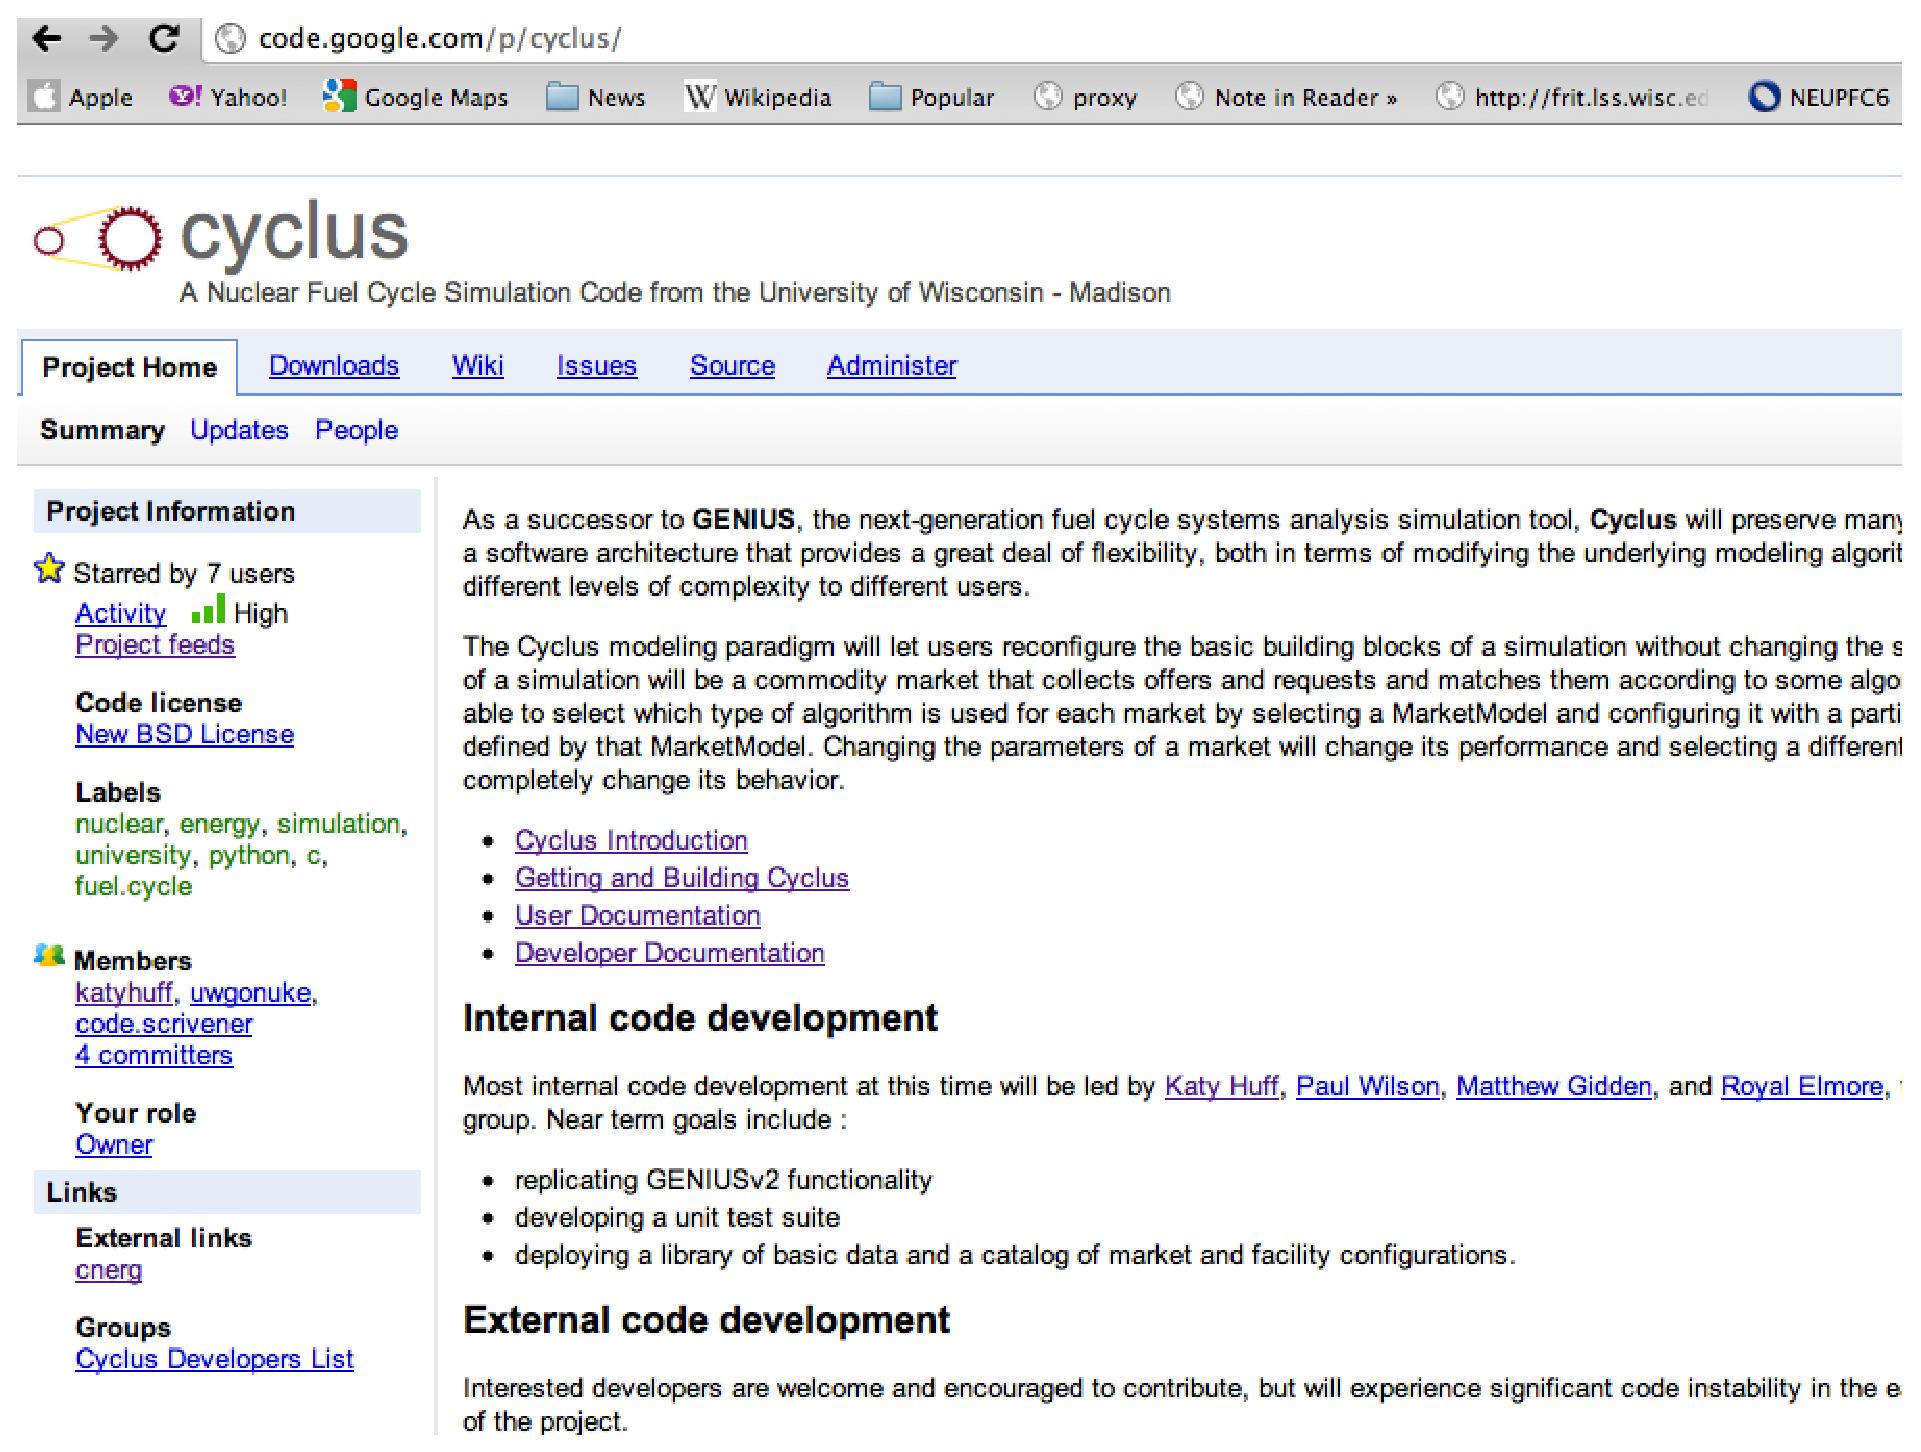
\includegraphics[height=6cm]{cyclushome.eps}
    \end{center}
    \caption{ Issues are created, assigned, and kept track of 
    alongside the code. } 
    \label{fig:issues}
  \end{figure}
\end{frame}
%---------------||||
\subsection{Testing Framework}
%||||---------------
\begin{frame}[ctb!]
  \frametitle{Testing Framework}
  A testing framework built on a cross-platform, multi-language build 
  system (CMake) allows developers to incorporate unit and integration 
  tests into their code before it is commited.
\end{frame}
%---------------||||
%||||---------------
\begin{frame}
  \frametitle{Summary}
  \begin{itemize}
    \item A modular architecture 
      \pause
    \item and open development paradigm 
      \pause
    \item support Cyclus users and developers  
      \pause
    \item at varying levels of sophistication and detail. 
  \end{itemize}
\end{frame}
%---------------||||
%||||---------------
\begin{frame}[allowframebreaks]
  \frametitle{References}
  \bibliographystyle{plain}
  {\footnotesize \bibliography{bibliography} }
\end{frame}
%---------------||||




\end{document}

%\begin{frame}[ctb!]
%  \frametitle{Openness}
%  Openness ensures transparency and lowers institutional technical 
%  obstacles to collaboration.
%\end{frame}


